\documentclass[UTF8,11pt,a4paper]{ctexart}

\usepackage[a4paper,margin=2.2cm]{geometry}
\usepackage{booktabs}
\usepackage{array}
\usepackage{tabularx}
\usepackage{enumitem}
\usepackage{xcolor}
\usepackage{hyperref}
\usepackage{fancyhdr}
\usepackage{titlesec}
\usepackage{setspace}
\usepackage{graphicx}
\usepackage{amsmath}
\usepackage{amssymb}
\usepackage{url}
\usepackage{float}
\usepackage{fancyvrb}

\hypersetup{
  colorlinks=true,
  linkcolor=blue!50!black,
  urlcolor=blue!50!black,
  pdftitle={低精度矩阵乘中的内积与外积：数据流、数值误差与架构决策},
  pdfauthor={},
  pdfsubject={Architecture study of inner-product and outer-product matrix multiplication},
  pdfkeywords={inner product, outer product, GEMM, FP8, accumulator, architecture}
}

\setmainfont{Times New Roman}
\setsansfont{Helvetica Neue}
\setmonofont{Menlo}
\setCJKmainfont{PingFang SC}
\setCJKsansfont{PingFang SC}
\setCJKmonofont{STHeiti}

\pagestyle{fancy}
\fancyhf{}
\lhead{内积与外积矩阵乘}
\rhead{\thepage}
\setlength{\headheight}{14pt}

\setlist[itemize]{leftmargin=2em}
\setlist[enumerate]{leftmargin=2.4em}
\setstretch{1.18}
\DefineVerbatimEnvironment{code}{Verbatim}{fontsize=\small}

\titleformat{\section}{\Large\bfseries}{\thesection}{0.8em}{}
\titleformat{\subsection}{\large\bfseries}{\thesubsection}{0.8em}{}
\titleformat{\subsubsection}{\normalsize\bfseries}{\thesubsubsection}{0.8em}{}

\newcommand{\ku}{\ensuremath{k_u}}

\title{\textbf{低精度矩阵乘中的内积与外积}\\
\large 数据流、数值误差与架构决策}
\author{}
\date{}

\begin{document}

\maketitle

\begin{abstract}
低精度矩阵乘单元常被粗略地划分为内积派与外积派，但这一二分在现代硬件中并不充分。对低精度
GEMM 而言，真正决定实现质量的往往不是标签本身，而是数据复用方式、局部归约深度以及
high-precision partial sum 的更新频率。本文围绕这一观察，对 inner-product primitive、
outer-product dataflow 和 tile-level MMA 三类组织方式进行统一分析。

本文首先从线性代数和数据流两种视角解释矩阵乘的内积式和外积式写法，并引入局部归约粒度 \ku{}，
用于刻画一个输出元素在一次高精度 psum 更新前已经融合了多少乘积项。随后，本文说明：
纯串行外积累加若以 $\hat{c}\leftarrow fl(\hat{c}+a_ib_i)$ 为最小更新单元，本质上对应
recursive summation；此时当前累计值的指数会在每一步都参与对齐和舍入，容易导致误差随累加深度放大。
相对地，inner-product primitive 或 grouped reduction 能把 accumulator 的作用从 product 级
推迟到 group 级，从而显著缓和 repeated alignment 与 swamping 问题。

在架构层面，本文表明：outer-product dataflow 的主要优势在于高复用、规则数据流和 dense GEMM
吞吐；inner-product primitive 的主要优势在于局部 K 归约语义清晰、数值路径更易控制；而现实中最稳妥
的实现通常是混合方案，即以 block outer-product 作为主数据流，再配合适中的 local dot-product depth。
基于公开矩阵原语，本文进一步说明 Arm SME 更偏显式 outer-product，Intel AMX 更偏显式 dot-product，
而 Tensor Core 与 DaVinci CUBE 则把软件接口停在 tile MMA 层，把真正的 inner/outer 组合留给微架构。

本文最终给出一个面向架构决策的结论：不存在脱离工作负载和数值 contract 的“内积必优”或“外积必优”；
真正应避免的是 \ku{} 过小、使高精度 accumulator 在 product 级频繁介入的纯串行外积累加。对现代低精度
dense GEMM，最稳妥的方向通常是 block outer-product dataflow 加适中的 local reduction depth。
\end{abstract}

\section{引言}

围绕矩阵乘单元到底应该做成“内积机”还是“外积机”，业界长期存在直觉化讨论。支持内积的一方强调：
dot-product primitive 更直接，局部 K 维归约更清楚，数值行为也更容易理解。支持外积的一方则强调：
一次读入一列 $A$ 和一行 $B$ 可以同时更新很多输出元素，因而更有利于数据复用和大规模阵列化实现。
这两类直觉都成立，但如果要把它们转化为真正的架构决策，仅靠抽象标签并不够。

现代低精度矩阵乘单元同时面临三类约束。第一类是吞吐和复用：在大 K、dense GEMM 场景下，
输入 tile 能否被充分复用，常常比单个乘法器是否紧凑更决定性能。第二类是数值：在 FP16/BF16/FP8
甚至 FP4 场景下，乘法器变便宜并不意味着累加一定便宜；很多实现真正昂贵的部分是 accumulator、
alignment、normalization 和 rounding。第三类是接口：软件究竟应看到 dot-product、outer-product
还是统一的 tile MMA，会反过来影响硬件需要承担多少实现自由度。

因此，本文关注的不是“谁在概念上更优”，而是一个更可操作的问题：\textbf{什么样的 inner/outer 组合，
能够同时兼顾数据复用、数值稳健性和实现代价。} 为此，本文给出三个层次的分析。

\begin{itemize}
  \item 在线性代数层面，说明内积式和外积式矩阵乘的等价关系，并给出直观例子与伪代码。
  \item 在数值分析层面，说明 pure outer accumulation 为什么会把高精度 psum 的指数影响引入到每一步，
  以及为什么 local reduction depth 是更有用的比较指标。
  \item 在架构层面，比较 inner-product primitive、outer-product dataflow 和 tile MMA，并给出
  针对不同工作负载和数值 contract 的选择框架。
  \item 在相关工作层面，把经典 systolic 论文、精确求和/点积算法以及近年的低精度 dot-product
  硬件一起纳入同一讨论框架。
\end{itemize}

\section{背景}

\subsection{矩阵乘的两种写法}

矩阵乘 $C=A\times B$ 可以写成两种等价形式：

\begin{align}
  C_{ij} &= \sum_k A_{ik}B_{kj}, \\
  C &\mathrel{+}= A_{:,k}B_{k,:}.
\end{align}

第一种写法强调每个输出元素都是一行和一列的内积；第二种写法强调每个 $k$ 步都可以把一列 $A$
和一行 $B$ 组合成一个 rank-1 更新。数学上二者等价，但在硬件上，它们鼓励完全不同的数据流组织：

\begin{itemize}
  \item 内积式写法更容易暴露为 dot-product 或 sum-of-products primitive。
  \item 外积式写法更容易组织成 rank-1 / rank-k update、systolic array 或 block outer-product
  数据流。
\end{itemize}

真正关键的问题不是“式子怎么写”，而是 partial sum 在哪一级被更新、以什么精度被更新、以及被更新多少次。

\subsection{一个直观例子}

设
\begin{equation}
  A=
  \begin{bmatrix}
    a_{11} & a_{12}\\
    a_{21} & a_{22}
  \end{bmatrix},
  \qquad
  B=
  \begin{bmatrix}
    b_{11} & b_{12}\\
    b_{21} & b_{22}
  \end{bmatrix}.
\end{equation}

则
\begin{equation}
  C=
  \begin{bmatrix}
    a_{11}b_{11}+a_{12}b_{21} & a_{11}b_{12}+a_{12}b_{22}\\
    a_{21}b_{11}+a_{22}b_{21} & a_{21}b_{12}+a_{22}b_{22}
  \end{bmatrix}.
\end{equation}

从内积视角看，$C_{11}$ 是 $[a_{11},a_{12}]$ 与 $[b_{11},b_{21}]$ 的点积；$C_{12}$ 是
$[a_{11},a_{12}]$ 与 $[b_{12},b_{22}]$ 的点积。
从外积视角看，可以先构造
\begin{equation}
  \begin{bmatrix}
    a_{11}\\ a_{21}
  \end{bmatrix}
  \begin{bmatrix}
    b_{11} & b_{12}
  \end{bmatrix}
\end{equation}
和
\begin{equation}
  \begin{bmatrix}
    a_{12}\\ a_{22}
  \end{bmatrix}
  \begin{bmatrix}
    b_{21} & b_{22}
  \end{bmatrix},
\end{equation}
再把这两个小矩阵相加。两种写法得到的是同一个结果，但前者强调“一个输出怎么形成”，后者强调
“一组输入能更新多少输出”。

\begin{figure}[H]
  \centering
  \begin{minipage}[t]{0.48\textwidth}
    \centering
    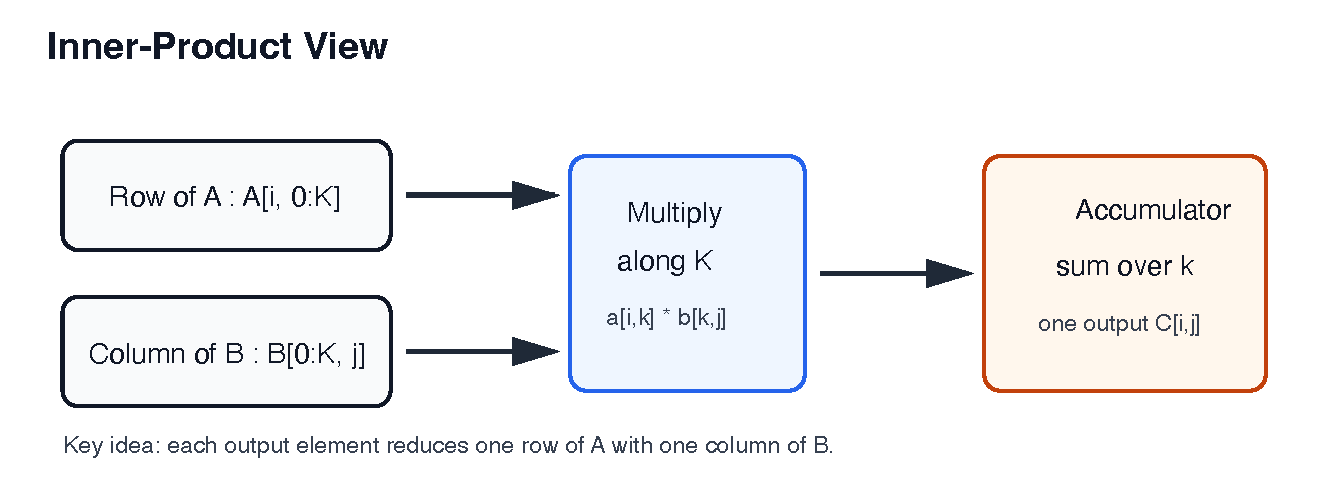
\includegraphics[width=\textwidth]{figures/inner-product-dataflow.pdf}
  \end{minipage}
  \hfill
  \begin{minipage}[t]{0.48\textwidth}
    \centering
    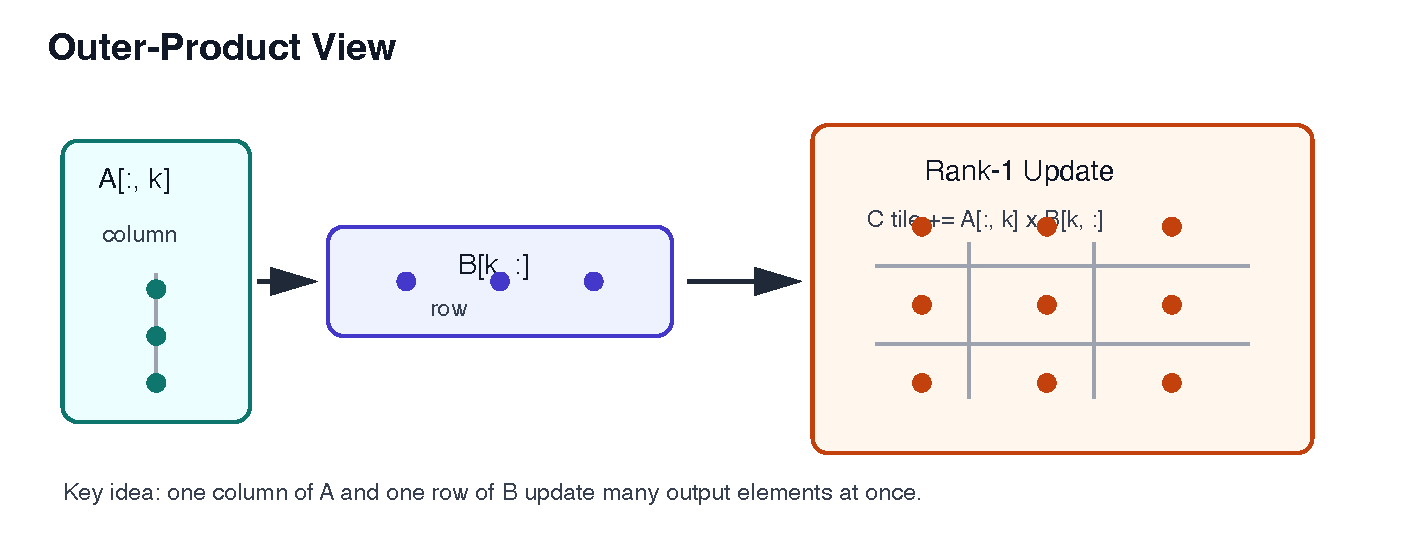
\includegraphics[width=\textwidth]{figures/outer-product-dataflow.pdf}
  \end{minipage}
  \caption{内积式与外积式矩阵乘的数据流示意。}
  \label{fig:inner-outer-new}
\end{figure}

\subsection{伪代码}

\noindent\textbf{Algorithm 1.} Inner-product GEMM
\begin{code}
for i in 0 .. M-1:
  for j in 0 .. N-1:
    acc = 0
    for k in 0 .. K-1:
      acc += A[i, k] * B[k, j]
    C[i, j] = acc
\end{code}

\noindent\textbf{Algorithm 2.} Outer-product GEMM
\begin{code}
initialize C to zero
for k in 0 .. K-1:
  a_col = A[:, k]
  b_row = B[k, :]
  for i in 0 .. M-1:
    for j in 0 .. N-1:
      C[i, j] += a_col[i] * b_row[j]
\end{code}

\noindent\textbf{Algorithm 3.} Tile MMA
\begin{code}
for each output tile (tm, tn):
  load C_tile
  for tk in K tiles:
    A_tile = load A[tm, tk]
    B_tile = load B[tk, tn]
    C_tile = MMA(A_tile, B_tile, C_tile)
  store C_tile
\end{code}

\subsection{为什么硬件关心 K 维、psum 和 accumulator}

矩阵乘的核心不是乘法本身，而是如何沿 K 维把乘积项归约到同一个输出元素。还没加完的中间结果，
本文统一称为 partial sum，简称 psum；负责保存和更新 psum 的寄存器、缓冲或阵列，统称为 accumulator。
对硬件而言，往往有三件事比“乘法器够不够多”更重要：

\begin{itemize}
  \item 一份输入能否被多个乘法器复用；
  \item psum 需要被读取、修改和写回多少次；
  \item 每次更新 psum 时，是否都需要较宽、较慢、较耗能的高精度加法路径。
\end{itemize}

\subsection{为什么低精度不等于累加一定便宜}

即使输入已经降到 FP16、FP8 甚至 FP4，累加仍然可能很贵。原因在于，多个乘积项相加后，
数值范围会快速增长。对定点而言，累加器通常至少要随着 $\log_2 K$ 增长位宽；对浮点而言，
不仅要处理 mantissa 相加，还要处理 exponent alignment、normalization 和 rounding。
因此，低精度矩阵乘真正的关键问题常常不是“能否做很多低精度乘法”，而是“能否减少 high-precision
psum 的更新频率”。

\subsection{经典工作如何看待内积、外积和规则数据流}

从体系结构史来看，outer-product 或 block outer-product 的吸引力并不是最近才出现的。
Kung 在 \emph{Why Systolic Architectures?} 中强调，规则数据流、局部互连和高数据复用是阵列式
计算获得高吞吐和可扩展性的核心原因 \cite{kung1982}。这条思路后来在矩阵乘上持续演化，并在
systolic array、TPU 以及后续张量单元中不断被重新实现 \cite{tpu,eyeriss}。从这个意义上说，
支持 outer-product dataflow 的最强论据并不在于“外积在数学上更高级”，而在于它更容易形成
高复用、局部通信和规则访存。

与此相对，数值分析领域很早就指出，求和顺序本身就是一等问题。Higham 对 floating-point summation
的系统分析揭示了 recursive summation、pairwise summation 和更高精度策略之间的误差差异 \cite{higham}；
Ogita、Rump 和 Oishi 则进一步给出了 Accurate Sum and Dot Product 算法，说明如何通过
error-free transformation 显著提高求和与点积的精度 \cite{ogita2005}。把这些结果翻译到硬件上，
它们实际上都在回答同一个问题：\textbf{局部 reduction 是不是只是实现细节，还是数值 contract 的一部分。}

\section{数值分析视角}

\subsection{局部归约粒度 \ku}

为了比较不同实现，本文定义局部归约粒度 \ku{}：
\begin{quote}
  \ku{} 表示单个输出元素在一次 high-precision psum 更新前，已经在本地融合的乘积项个数。
\end{quote}

\begin{itemize}
  \item $\ku=1$ 表示几乎每个乘积都直接更新 psum。
  \item $\ku=2,4,8,16$ 表示先在局部做小规模 dot 或 SoP，再更新 psum。
  \item $\ku=K_{tile}$ 表示几乎把整个局部 K 归约都放在高精度更新之前完成。
\end{itemize}

若完整归约长度为 $K$，则单个输出元素触发高精度累加的次数近似为
\begin{equation}
N_{\text{acc}} \approx \frac{K}{\ku}.
\end{equation}

\subsection{纯串行外积累加为什么更危险}

这里必须区分 \textbf{outer-product dataflow} 和 \textbf{pure outer accumulation}。
前者只是在说输入和输出的复用方式；后者则是在说最小更新单元。如果最小更新单元是
\begin{equation}
  \hat{c}_{t+1} = fl(\hat{c}_t + p_t), \qquad p_t = a_t b_t,
\end{equation}
那么它本质上就是 recursive summation。此时，当前累计值 $\hat{c}_t$ 的指数会在每一步都参与
alignment，新的乘积 $p_t$ 需要不断按照 $\hat{c}_t$ 的量级右移并舍入。若 $\hat{c}_t$ 已经很大，
而 $p_t$ 相对较小，就会出现 swamping，甚至满足 $fl(\hat{c}_t + p_t)=\hat{c}_t$。

Higham 对 floating-point summation 的经典分析指出，recursive summation 的误差常数与归约长度
$K$ 近似线性相关，而 pairwise summation 的误差常数更接近 $\log K$ 量级 \cite{higham}。
从架构角度看，这一结论的含义是：如果 accumulator 在 product 级反复介入，那么当前 psum 的指数会反复
支配新乘积的对齐位置；若先做 grouped reduction 或 local dot，再把结果送进 accumulator，
则高精度 psum 只在 group 级起作用。

\subsection{为什么局部 dot/reduction 在数域上有意义}

这也是 fused dot-product 单元存在的根本原因。Lutz 等人的 FP8-DOT4 工作强调，4-way dot product
在进入 FP32 accumulation 之前不做中间 rounding，从而把四个乘积与 accumulator 的交互压缩成一次
\cite{lutz2024}。Exact dot product 则把这一思想推到极致，在最终输出前尽量避免中间舍入 \cite{exactdot}。

因此，outer dataflow 内部再引入 local dot/reduction，不是“把外积偷偷改成内积”，而是有明确数值意义的：

\begin{itemize}
  \item 它保留外积式数据复用和 tile 更新的优势；
  \item 它避免最差形式的 product 级高频 $\hat{c}\leftarrow fl(\hat{c}+p)$；
  \item 它让高精度 accumulator 尽量在 group 级而不是 product 级参与对齐和舍入。
\end{itemize}

\subsection{扩展路线：精确点积、共享尺度和专用 dot-product ISA}

除了最基础的 grouped reduction，文献中还有几条更激进或更工程化的路线。第一类是更强的数值路径。
Accurate Sum and Dot Product \cite{ogita2005} 与 exact dot product \cite{exactdot} 代表了两个极端：
前者强调算法级的高精度变换，后者强调用超宽 accumulator 尽可能推迟最终舍入。它们共同说明，
如果设计目标是极强的数值 contract，那么“在哪一级舍入”本身就会变成一条主导架构的约束。

第二类是把共享尺度或 block scaling 与 dot-product primitive 直接绑定。Microscaling 数据格式
提出之后，近期的 MXDOTP 工作把 MXFP8 的 block scale 与 dot-product unit 直接耦合，说明在低位宽
浮点里，局部 dot primitive 不仅是 reduction primitive，也可以成为 scale application 的自然载体
\cite{mxdotp,mx}. 这类工作意味着，inner-product primitive 的价值并不限于“便于归约”，还包括
更容易把 block scale、shared exponent 和 accumulation contract 打包成一个统一单元。

第三类是面向极低位宽神经网络的专用点积加速器。MiniFloat-NN 中的 ExSdotp 单元专门针对
dot-product 的精度损失做了扩展，实现上通过专用扩展字段和修改后的累加逻辑减少精度损失与饱和风险
\cite{exsdotp}。这说明在低比特浮点场景里，inner-product primitive 之所以反复出现，并不只是因为
“点积更像课本”，而是因为它给了设计者一个更自然的位置去放置 scale、carry、extra bits 和 rounding policy。

\section{架构比较}

\subsection{Inner-product primitive 的优势与代价}

采用 inner-product primitive 时，局部 K 归约语义非常明确。其优势主要在于：

\begin{itemize}
  \item 软件语义直接，对一个输出元素的形成方式理解清楚；
  \item 局部 reduction 边界清楚，更容易把 accumulator 的介入控制在 dot-product 级；
  \item 对数值 contract 较敏感时，更容易给出明确的误差路径。
\end{itemize}

但其代价也很明显：

\begin{itemize}
  \item 如果要提升 \ku{}，SoP datapath 会迅速变宽；
  \item dot-product lane 的输入复用通常不如 block outer-product 自然；
  \item 大规模阵列化时，更容易遇到输入广播和局部 reduction 网络的代价。
\end{itemize}

\subsection{Outer-product dataflow 的优势与代价}

outer-product dataflow 的主要优势是 dense GEMM 场景下的高复用和规则数据流。
一次读入一列 $A$ 和一行 $B$，就能同时更新一片输出 tile；这与 systolic array 和大规模矩阵阵列的组织方式
高度一致 \cite{blis,tpu,eyeriss}。

但 outer-product 的风险不在数据流本身，而在数值最小粒度。如果实现退化为 $\ku=1$ 的纯串行外积累加，
那么误差、能耗和时序压力都会被推到 high-precision accumulator 上。因此，outer-product 真正成立的前提是：
\textbf{外积只作为主数据流，而不是作为 product 级高精度更新规则。}

\subsection{Tile MMA 作为接口层折中}

许多现代设计并不把 inner 或 outer 直接暴露给软件，而是把接口停在 tile MMA：
\begin{equation}
  D = A\times B + C.
\end{equation}

这种接口的价值在于，它允许软件获得统一抽象，同时把 inner/outer 的真正组合留给微架构。
从这个角度看，tile MMA 并不是第三种完全独立的数学形式，而是一个实现自由度更高的接口层折中。

\subsection{公开矩阵原语的定位}

公开矩阵原语可以作为一个很好的参照系：

\begin{itemize}
  \item Arm SME 在 ISA 层显式暴露 outer-product accumulate \cite{smeintro,smeinst}。
  \item Intel AMX 在 ISA 层显式暴露 dot-product tile primitive \cite{amxbf16,amxsample}。
  \item NVIDIA Tensor Core 和 DaVinci CUBE 则在软件接口上更像 tile MMA，真正的数据流和局部归约方式由微架构决定 \cite{ptxisa,cutlass,ascendmmad,davinci}。
\end{itemize}

\begin{figure}[H]
  \centering
  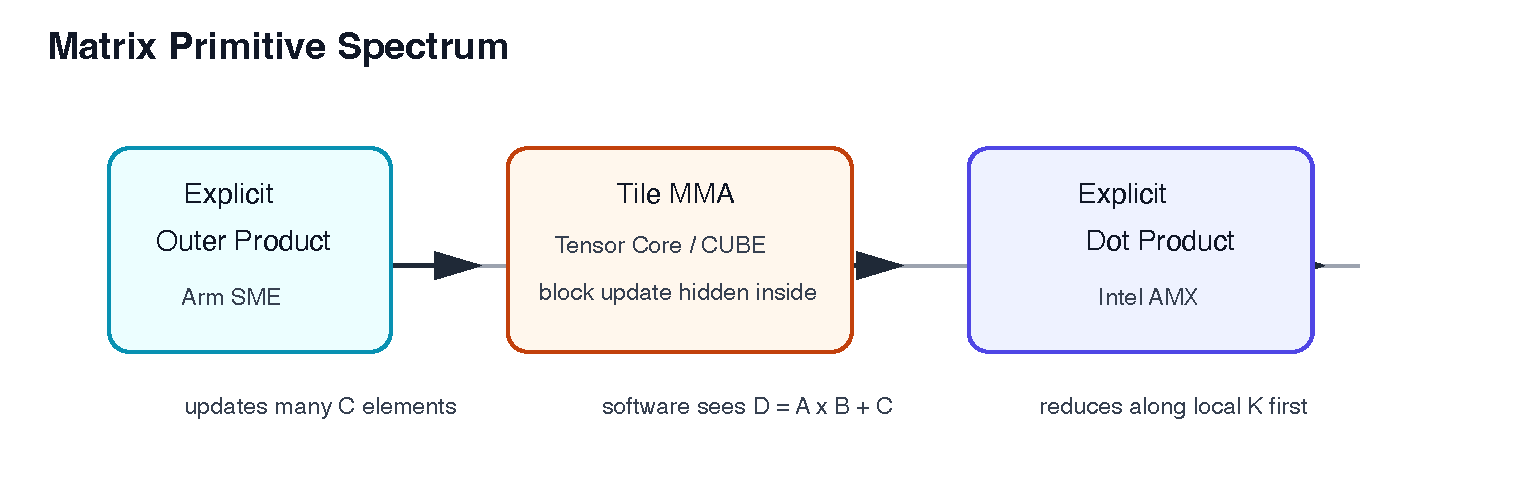
\includegraphics[width=0.9\textwidth]{figures/tile-mma-spectrum.pdf}
  \caption{公开矩阵原语的一个直观谱系。}
  \label{fig:spectrum-new}
\end{figure}

\noindent\textbf{Algorithm 4.} SME-style outer-product tile update
\begin{code}
load ZA tile
for each k-step:
  a_vec = load vector from A
  b_vec = load vector from B
  ZA += outer_product(a_vec, b_vec)
store ZA tile
\end{code}

\noindent\textbf{Algorithm 5.} AMX-style dot-product tile update
\begin{code}
load dst tile
for each local K chunk:
  a_tile = load tile from A
  b_tile = load tile from B
  dst += dot_product_reduce(a_tile, b_tile)
store dst tile
\end{code}

\subsection{文献中的共识与分歧}

把这些经典与近期工作放在一起，可以看到一个比较稳定的共识。共识在于：无论是 systolic 路线、
dot-product 路线还是 exact accumulation 路线，大家最终都在处理同一个问题，即如何在复用、局部归约
和高精度 psum 更新之间取得平衡。分歧则主要出现在“应把复杂度放在哪一级”：outer-product 路线倾向于把
复杂度放在数据流组织和 psum 管理上，dot-product 路线倾向于把复杂度放在局部 SoP datapath 和 reduction
primitive 上，而 exact/accurate 路线则愿意把复杂度进一步推到 accumulator 本身。

因此，相关工作给本文最重要的启发并不是哪一派“获胜”，而是：任何脱离 \ku{}、舍入位置、block scale、
以及工作负载几何形状的 inner/outer 讨论，都很容易变成失真的标签之争。真正高质量的设计，往往是先选定
主数据流，再选定 local reduction depth，最后再决定 high-precision psum 在哪一级介入。

\section{架构决策框架}

\subsection{三个首先要问的问题}

真正做方案选择时，最有用的往往不是贴标签，而是回答以下三个问题：

\begin{enumerate}
  \item \textbf{主矛盾是复用还是局部归约？}
  大 K dense GEMM 常常优先关注输入复用和规则数据流；小 K 或强调局部语义的场景更关心 reduction primitive 本身。
  \item \textbf{能接受多高的 high-precision psum 更新频率？}
  如果数值、能耗或时序预算不允许 accumulator 在 product 级频繁介入，就必须提高 \ku{}。
  \item \textbf{软件接口需要暴露什么层级的抽象？}
  若希望软件看到 outer-product tile update，则更偏 SME；若希望软件看到 dot product，则更偏 AMX；
  若希望保留硬件实现自由度，则更偏 tile MMA。
\end{enumerate}

\subsection{决策表}

\begin{table}[H]
  \centering
  \caption{面向架构决策的 inner / outer 选择建议}
  \label{tab:decision-new}
  \begin{tabularx}{\textwidth}{>{\raggedright\arraybackslash}p{3.0cm} >{\raggedright\arraybackslash}p{3.3cm} >{\raggedright\arraybackslash}X}
    \toprule
    场景或约束 & 更合适的方向 & 主要理由 \\
    \midrule
    大 K、dense GEMM、规则 tile & block outer-product + local reduction & 输入复用高，数据流规则；但必须避免 $\ku=1$ 的 product 级高频 psum 更新 \\
    小 K、需要明确局部 K 归约语义 & inner-product primitive / grouped dot product & accumulator 介入次数更少，数值路径更可控，软件语义也更直接 \\
    既要高吞吐又要保留实现自由度 & tile MMA & 软件看到统一的 $D=A\times B+C$，硬件可自行组合 outer dataflow 与 local reduction \\
    FP16/BF16/FP8，精度风险敏感 & 避免纯串行 outer accumulation & 应优先提高 \ku{}，把 sequential accumulation 改成 grouped 或 tree-style accumulation \\
    极度强调高精度 contract & dot-product / exact-style accumulation & 舍入点更少，误差边界更容易分析，但面积和时序代价更高 \\
    \bottomrule
  \end{tabularx}
\end{table}

\subsection{本文的最终判断}

基于全文分析，本文给出以下判断：

\begin{itemize}
  \item 不存在脱离工作负载和数值 contract 的“内积必优”或“外积必优”。
  \item 对现代低精度 dense GEMM，最稳妥的路线通常是 \textbf{block outer-product dataflow + 适中的 local reduction depth}。
  \item 真正应该避免的是 \textbf{\ku{} 过小的纯串行外积累加}，因为它会让高精度 accumulator 在 product 级反复介入。
  \item 如果必须在“纯内积”和“纯外积”之间二选一，本文更反对的是纯串行外积累加；若允许现实工程中的混合方案，
  则更支持外积主数据流配局部 dot/reduction。
\end{itemize}

\section{结论}

内积和外积不是非此即彼的教条选择，而是矩阵乘实现空间中的两个极端视角。inner-product primitive
的强项在于局部归约语义清晰、数值路径更容易控制；outer-product dataflow 的强项在于高复用、规则数据流
和 dense GEMM 吞吐。现代矩阵单元之所以看起来经常“既像内积又像外积”，恰恰说明现实最优点通常位于二者之间。

对架构设计而言，真正决定好坏的不是标签，而是是否能够同时处理好三件事情：数据复用、局部归约深度和
high-precision psum 更新频率。只要 local reduction depth 足够，outer-product dataflow 完全可以
在数值上站得住；反之，若退化为 product 级高频 $\hat{c}\leftarrow fl(\hat{c}+p)$，则 outer-product
方案会在精度和能效上同时受损。

因此，本文建议把“inner vs outer”的讨论从抽象阵营之争，转化为更具体的架构问题：
\begin{quote}
  选择什么样的主数据流，配置多大的局部归约深度，并让 accumulator 在哪一级介入。
\end{quote}
只有在这个层面上，内积和外积的比较才真正能为架构决策服务。

\begin{thebibliography}{99}

\bibitem{blis}
Tyler M. Smith, Robert A. van de Geijn, M. Smelyanskiy, Jeff R. Hammond, and Field G. Van Zee.
\newblock Analytical Modeling Is Enough for High-Performance BLIS.
\newblock \emph{ACM Transactions on Mathematical Software}, 2018.
\newblock \url{https://www.cs.utexas.edu/~flame/pubs/flawn74.pdf}

\bibitem{kung1982}
H. T. Kung.
\newblock Why Systolic Architectures?
\newblock \emph{Computer}, 15(1):37--46, 1982.
\newblock \url{https://www.eecs.harvard.edu/~htk/publication/1982-kung-why-systolic-architecture.pdf}

\bibitem{tpu}
Norman P. Jouppi et al.
\newblock In-Datacenter Performance Analysis of a Tensor Processing Unit.
\newblock In \emph{ISCA}, 2017.
\newblock \url{https://arxiv.org/abs/1704.04760}

\bibitem{eyeriss}
Yu-Hsin Chen, Tushar Krishna, Joel S. Emer, and Vivienne Sze.
\newblock Eyeriss: An Energy-Efficient Reconfigurable Accelerator for Deep Convolutional Neural Networks.
\newblock \emph{IEEE Journal of Solid-State Circuits}, 2017.
\newblock \url{https://people.csail.mit.edu/emer/media/papers/2016.06.isca.eyeriss_architecture.pdf}

\bibitem{lutz2024}
David Raymond Lutz, Anisha Saini, Mairin Kroes, Thomas Elmer, and Harsha Valsaraju.
\newblock Fused FP8 4-Way Dot Product With Scaling and FP32 Accumulation.
\newblock In \emph{ARITH}, 2024.
\newblock \url{https://www.ac.uma.es/arith2024/papers/Fused%20FP8%204-Way%20Dot%20Product%20with%20Scaling%20and%20FP32%20Accumulation.pdf}

\bibitem{exactdot}
Jack Koenig.
\newblock A Hardware Accelerator for Computing an Exact Dot Product.
\newblock UC Berkeley Technical Report UCB/EECS-2018-51, 2018.
\newblock \url{https://www2.eecs.berkeley.edu/Pubs/TechRpts/2018/EECS-2018-51.pdf}

\bibitem{higham}
Nicholas J. Higham.
\newblock The Accuracy of Floating Point Summation.
\newblock \emph{SIAM Journal on Scientific Computing}, 14(4):783--799, 1993.
\newblock \url{https://nhigham.com/wp-content/uploads/2023/10/high93s.pdf}

\bibitem{ogita2005}
Takeshi Ogita, Siegfried M. Rump, and Shin'ichi Oishi.
\newblock Accurate Sum and Dot Product.
\newblock \emph{SIAM Journal on Scientific Computing}, 26(6):1955--1988, 2005.
\newblock \url{https://waseda.elsevierpure.com/en/publications/accurate-sum-and-dot-product}

\bibitem{smeintro}
Arm.
\newblock Arm Scalable Matrix Extension Introduction.
\newblock Arm developer documentation.
\newblock \url{https://developer.arm.com/documentation/109246/latest/}

\bibitem{smeinst}
Arm.
\newblock FMOPA, BFMOPA, and related SME instructions.
\newblock Arm Architecture Reference Manual for A-profile architecture supplement.
\newblock \url{https://developer.arm.com/documentation/ddi0616/latest/}

\bibitem{amxbf16}
Intel.
\newblock \_tile\_dpbf16ps: Compute dot-product of BF16 pairs in tiles.
\newblock Intel oneAPI DPC++/C++ Compiler Developer Guide and Reference.
\newblock \url{https://www.intel.com/content/www/us/en/docs/dpcpp-cpp-compiler/developer-guide-reference/current/tile-dpbf16ps.html}

\bibitem{amxsample}
Intel.
\newblock Advanced Matrix Extensions Intrinsics Functions.
\newblock Intel developer article and code sample.
\newblock \url{https://www.intel.com/content/www/us/en/developer/articles/code-sample/advanced-matrix-extensions-intrinsics-functions.html}

\bibitem{ptxisa}
NVIDIA.
\newblock Parallel Thread Execution ISA: Matrix multiply-accumulate instructions.
\newblock NVIDIA documentation.
\newblock \url{https://docs.nvidia.com/cuda/parallel-thread-execution/}

\bibitem{cutlass}
NVIDIA.
\newblock CUTLASS GEMM API.
\newblock NVIDIA documentation.
\newblock \url{https://docs.nvidia.com/cutlass/media/docs/cpp/gemm_api.html}

\bibitem{ascendmmad}
Vendor.
\newblock Mmad matrix multiply-accumulate API.
\newblock Ascend C API documentation.
\newblock \url{https://www.hiascend.com/document/detail/zh/CANNCommunityEdition/800alpha003/apiref/ascendcopapi/atlasascendc_api_07_0249.html}

\bibitem{davinci}
Marc Salvad\'o, Josep L. Briz, and Miquel Moret\'o.
\newblock Exploring the DaVinci Machine Learning Accelerator Architecture via Software-Hardware Simulation.
\newblock In \emph{International Conference on High Performance Computing \& Simulation Workshops}, 2021.
\newblock \url{https://webdocs.cs.ualberta.ca/~csalvado/publication/2021-pooling-acceleration-in-davinci/pooling-acceleration-in-davinci.pdf}

\bibitem{mxdotp}
Gamze\. Islamo\u{g}lu, Luca Bertaccini, Arpan Suravi Prasad, Francesco Conti, Angelo Garofalo, and Luca Benini.
\newblock MXDOTP: A RISC-V ISA Extension for Enabling Microscaling (MX) Floating-Point Dot Products.
\newblock arXiv:2505.13159, 2025.
\newblock \url{https://arxiv.org/abs/2505.13159}

\bibitem{exsdotp}
Giacomo G. Cazzola, Luca Colagrande, Francesco Conti, and Luca Benini.
\newblock MiniFloat-NN: Reducing Hardware Cost of On-Device Training with Low-Precision Floating-Point.
\newblock arXiv:2209.05400, 2022.
\newblock \url{https://arxiv.org/abs/2209.05400}

\end{thebibliography}

\end{document}
